%\documentclass[spanish]{beamer}

\documentclass{beamer}
\usepackage{pgf,pgfpages}
%\pgfpagesuselayout{4 on 1}[letterpaper,landscape,border shrink=0.5in]
\usepackage{algorithm,algorithmic}
%\usepackage{algorithm,algorithmicx}
%\usepackage[noend]{algpseudocode}
\usepackage{listings}
\lstset{basicstyle=\ttfamily,
	showstringspaces=false,
	commentstyle=\color{red},
	literate={á}{{\'a}}1
	{ã}{{\~a}}1
	{é}{{\'e}}1
	{ó}{{\'o}}1
	{í}{{\'i}}1
	{ñ}{{\~n}}1
	{¡}{{!`}}1
	{¿}{{?`}}1
	{ú}{{\'u}}1
	{Í}{{\'I}}1
	{Ó}{{\'O}}1
}

\usepackage{beamerthemesplit}
\usepackage{color}
\usepackage[utf8]{inputenc}
\usepackage[spanish]{babel}
%\usepackage[latin1]{inputenc}
%\usepackage[pdftex]{graphicx}
%\usepackage{algorithm}
%\usepackage{algorithmic-C}
%\usepackage{algorithmic}
\usepackage{amsthm}
\usepackage{multicol}
\usepackage{multirow}
\usepackage{fancyvrb,relsize}
\usepackage{hhline}
\usepackage{tikz}
\usetikzlibrary{trees, shapes, calc}
\newcommand{\inputTikZ}[2]{%
	\scalebox{#1}{\input{#2}}
}

\usetheme{Warsaw} %Gueno
%\usetheme{Darmstadt} %OK!
% \usetheme{Frankfurt} %OK!
%\usetheme{Goettingen}
%\usetheme{Dresden}
%\usetheme{JuanLesPins} %OK!!
%\usetheme{Marburg}
%\usetheme{Montpellier}
%\usetheme{Rochester} %sobrio
%\usetheme{Singapore}
%\usetheme{Szeged}

%\usecolortheme{albatross}
%\usecolortheme{seahorse}
%\usecolortheme{beetle}
%\usecolortheme{crane}
%\usecolortheme{dolphin}
%\usecolortheme{dove}
%\usecolortheme{fly}
%\usecolortheme{lily} %Gueno
\usecolortheme{orchid}%Gueno
%\usecolortheme{rose}
%\usecolortheme{seagull}
%\usecolortheme{whale}


\DefineVerbatimEnvironment%
      {VerbatimNN}%
      {Verbatim}%
      {fontsize=\relsize{-1}}
\DefineVerbatimEnvironment%
      {VerbatimNNN}%
      {Verbatim}%
      {fontsize=\relsize{-2}}

\DefineVerbatimEnvironment%
      {VerbatimPseudo}%
      {Verbatim}%
      {numbers=left, fontsize=\relsize{-1}}
\DefineVerbatimEnvironment%
      {VerbatimPseudoReduced}%
      {Verbatim}%
      {numbers=left, fontsize=\relsize{-2}}
\DefineVerbatimEnvironment%
      {VerbatimPseudoReduced2}%
      {Verbatim}%
      {numbers=left, fontsize=\relsize{-3}}
\DefineVerbatimEnvironment%
      {VerbatimC}%
      {Verbatim}%
      {commandchars=@ªº, numbers=left, fontsize=\relsize{-1}}
\DefineVerbatimEnvironment%
      {VerbatimReducedC}%
      {Verbatim}%
      {commandchars=@ªº, numbers=left, fontsize=\relsize{-2}}
\DefineVerbatimEnvironment%
      {VerbatimReduced2C}%
      {Verbatim}%
      {commandchars=@ªº, numbers=left, fontsize=\relsize{-3}}



%\AtBeginSubsection[]
%{
% \begin{frame}
% \frametitle{Sinopsis}
% Aqui decides: cada seccion y subseccion:
% \tableofcontents[currentsection,currentsubsection]
 %O solamente la seccion (Solo uno de ellos)
%\tableofcontents[currentsection]
% \end{frame}
%}

% Si quieres que todo por default aparezca de poco en poco
% descomenta esta linea
%\beamerdefaultoverlayspecification{<+->}

\setbeamertemplate{footline}{\hfill\insertframenumber/\inserttotalframenumber}
\setbeamertemplate{navigation symbols}{}

\setbeamercovered{transparent}

\title{ELO320 - Estructuras de Datos y Algoritmos\\Introducción a C\\Punteros}
%\subtitle{Ingeniería Civil Telemática UTFSM}
\author{Dr. Nicolás Gálvez R.\\{\small nicolas.galvez@usm.cl}}
\institute{Ing. Civil Telemática - Departamento de Electrónica}
\titlegraphic{
\includegraphics[scale=.13]{images/logoutfsm}}
\date{1er Semestre 2025}

\begin{document}

\frame{\titlepage}

%\section*{Sinopsis}
%\frame{  \frametitle{Sinopsis}\tableofcontents[pausesections]}
%
%
\part{Clase Activa}
\section{Clase Activa}
\begin{frame}[fragile]{Clase Activa: Módulo 1}
\begin{exampleblock}{Ejercicio 1.1}
Cree una función que reciba como parámetro un arreglo de enteros y el tamaño de éste, y luego muestre por pantalla los valores almacenados en dicho arreglo. Puede usar una de las dos siguientes declaraciones:
\begin{lstlisting}[language=C, basicstyle=\scriptsize]
void imprimir_datos(int arreglo[], int tam);

void imprimir_datos(int * arreglo, int tam);
\end{lstlisting}
\end{exampleblock}

{\tiny Aprendemos: Definir un arreglo, recorrer un arreglo, rellenar un arreglo. Paso por referencia.}
\end{frame}

\begin{frame}[fragile]{Clase Activa: Módulo 1}
\begin{exampleblock}{Ejercicio 1.2}
Cree una función que reciba como parámetro un arreglo de enteros y el tamaño de éste, y luego muestre por pantalla los valores almacenados en dicho arreglo. \textbf{No puede usar el operador []}. Puede usar una de las dos siguientes declaraciones:
\begin{lstlisting}[language=C, basicstyle=\scriptsize]
void imprimir_datos_2(int arreglo[], int tam);

void imprimir_datos_2(int * arreglo, int tam);
\end{lstlisting}
\end{exampleblock}

{\tiny Aprendemos: Aritmética de Punteros.}
\end{frame}


\begin{frame}[fragile]{Clase Activa: Módulo 2}
\begin{exampleblock}{Ejercicio 2.1}
Cree una función que reciba como parámetro un arreglo de enteros y el tamaño de éste, y luego calcule el promedio entre todos los valores almacenados en dicho arreglo. Puede usar una de las dos siguientes declaraciones:
\begin{lstlisting}[language=C, basicstyle=\scriptsize]
float promedio(int arreglo[], int tam);

float promedio(int * arreglo, int tam);
\end{lstlisting}
\end{exampleblock}

{\tiny Aprendemos: Operar sobre un arreglo, recorrer un arreglo.}
\end{frame}

\begin{frame}[fragile]{Clase Activa: Módulo 2}
\begin{exampleblock}{Ejercicio 2.2}
Cree una función que reciba como parámetro un arreglo de enteros, el tamaño de éste, y una variable que contendrá el promedio de éste arreglo. La función debe calcular el promedio entre todos los valores almacenados en dicho arreglo. El promedio debe permanecer fuera de la función. \textbf{No puede usar variables globales}. Puede usar una de las dos siguientes declaraciones:
\begin{lstlisting}[language=C, basicstyle=\scriptsize]
void promedio(int arreglo[], int tam, float * prom);

void promedio(int * arreglo, int tam, float * prom);
\end{lstlisting}
\end{exampleblock}

{\tiny Aprendemos: Operar sobre un arreglo, Paso de parámetro por referencia.}
\end{frame}

\begin{frame}[fragile]{Clase Activa: Módulo 3}
Analice y explique qué realiza el siguiente código:
\begin{exampleblock}{Ejercicio 3.1}
\begin{lstlisting}[language=C, basicstyle=\scriptsize, escapeinside={|}{|}]
#include<stdio.h>

void swap(int a, int b){
	int temp;
	temp = a;
	a = b;
	b = temp;
}

int main(){
	int x=2, y=3;
	swap(x,y);
	printf("x: |\%|d, y: |\%|d\n", x, y); // ¿Qué imprime?
	return 0;
}
\end{lstlisting}
\end{exampleblock}

{\tiny Aprendemos: Paso de parámetro por valor.}
\end{frame}


\begin{frame}[fragile]{Clase Activa: Módulo 3}
Analice y explique qué realiza el siguiente código:
\begin{exampleblock}{Ejercicio 3.2}
\begin{lstlisting}[language=C, basicstyle=\scriptsize, escapeinside={|}{|}]
#include<stdio.h>

void swap(int *a, int *b){ 
	int temp;
	temp = *a; 
	*a = *b
	*b = temp;
}

int main(){
	int x=2, y=3;
	swap(|\&|x,|\&|y);
	printf("x: |\%|d, y: |\%|d\n", x, y); //¿Qué imprime?
	return 0;
}
\end{lstlisting}
\end{exampleblock}

{\tiny Aprendemos: Paso de parámetro por valor.}
\end{frame}


\begin{frame}[fragile]{Clase Activa: Módulo 3}
Analice y explique qué realiza el siguiente código:
\begin{exampleblock}{Ejercicio 3.3}
\begin{lstlisting}[language=C, basicstyle=\scriptsize, escapeinside={|}{|}]
#include<stdio.h>

void swap(int *a, int *b){
	int *temp;
	temp = a; 
	a = b; 
	b = temp;
}

int main(){
	int x=2, y=3;
	swap(|\&|x,|\&|y);
	printf("x: |\%|d, y: |\%|d\n", x, y); //¿Qué imprime?
	return 0;
}
\end{lstlisting}
\end{exampleblock}

{\tiny Aprendemos: Paso de parámetro por valor.}
\end{frame}

\begin{frame}[fragile]{Clase Activa: Módulo 3}
Analice y explique qué realiza el siguiente código:
\begin{exampleblock}{Ejercicio 3.4}
\begin{lstlisting}[language=C, basicstyle=\scriptsize, escapeinside={|}{|}]
#include<stdio.h>

void swap(int *a, int *b){
	int *temp;
	temp = a; 
	*a = *b; 
	*b = *temp;
}

int main(){
	int x=2, y=3;
	swap(|\&|x,|\&|y);
	printf("x: |\%|d, y: |\%|d\n", x, y); //¿Qué imprime?
	return 0;
}
\end{lstlisting}
\end{exampleblock}

{\tiny Aprendemos: Paso de parámetro por valor.}
\end{frame}


\part{Punteros}
\begin{frame}
\centering \Huge Información de Vital Importancia para la Clase Activa\footnote{Depende exclusivamente de uds. leerla y comprenderla.}.
\end{frame}

\section{Memoria en C}

\begin{frame}
\frametitle{Programa en Memoria}
  \begin{itemize}
  \item \emph{Ejecutar}: llevar un programa (binario) a memoria.
  \item \emph{Variables y Constantes}: espacios de que se asignan y liberan
en memoria
  \item \emph{Ciclo de vida}: cuando se crea y destruye una variable
  \item \emph{Ámbito}: qué código tiene acceso a la variable
  \end{itemize}
\vspace{-.2cm}
\begin{center}
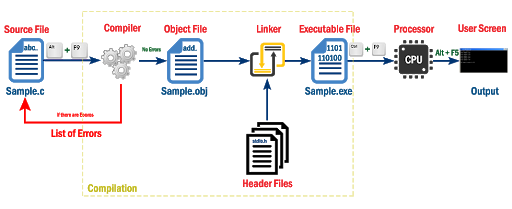
\includegraphics[width=.85\linewidth]{images/compila}
\end{center}
\vspace{-.2cm}

\end{frame}

\subsection{Taxonomía de la Memoria}
\frame[containsverbatim]
{
\frametitle{Taxonomía de la memoria}

Segmentos de memoria:
\begin{center}
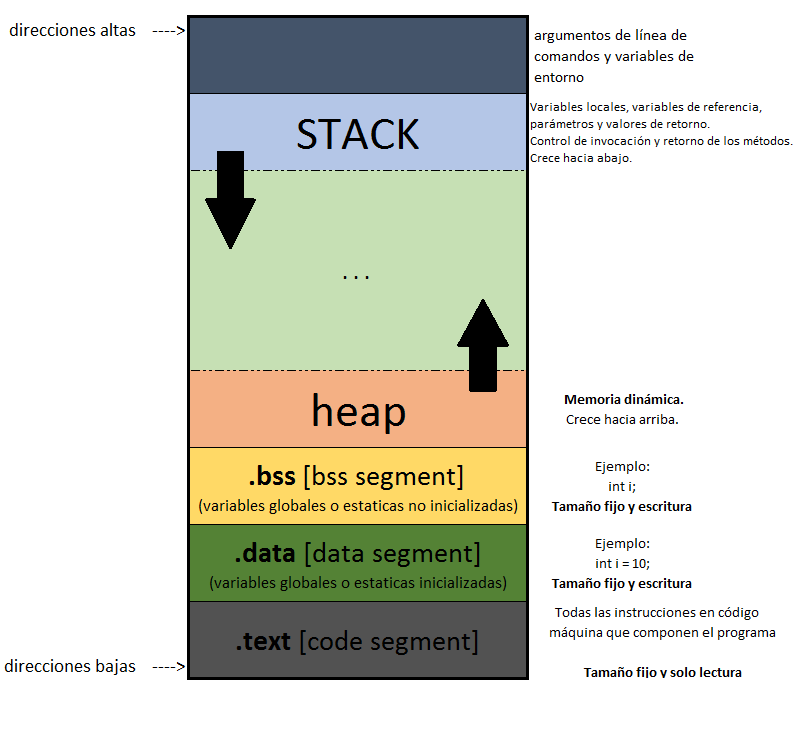
\includegraphics[width=.7\linewidth]{images/memoriastack}
\end{center}
}

\frame[containsverbatim]
{
\frametitle{Taxonomía de la memoria}
Segmentos de memoria:
  \begin{enumerate}
\item \textbf{Memoria text o de código}.
\item \textbf{Memoria static o estática}.
\item \textbf{Memoria heap}. 
\item \textbf{Memoria stack o call stack}. 
\end{enumerate} 
}

\frame[containsverbatim]
{
\frametitle{\textbf{Memoria text}}
\Large Donde el programa compilado se mantiene en memoria.
}

\frame[containsverbatim]
{
\frametitle{\textbf{Memoria static}}
\large Mantiene variables globales y estáticas.
\bigskip 

\large Ligado estático: variables (y valores) en la memoria hasta que programa termina. 
}

\frame[containsverbatim]
{
\frametitle{\textbf{Memoria heap}}
\large Permite al programador crear y eliminar objetos de memoria dinámicamente. 
\bigskip

\large Son referenciadas indirectamente mediante \textbf{punteros} y/o \textbf{referencias}.
}

\frame[containsverbatim]
{
\frametitle{\textbf{Memoria stack}}
\large Área dinámica de memoria donde se guardan las variables locales y la información de las funciones.
\bigskip

\large Permite mantener objetos que se asignan y liberan automáticamente en ambiente de ejecución.
\bigskip

\large Manejado \textbf{automáticamente} por el compilador.
}

\subsection{Tipos de variables}
\frame[containsverbatim]
{
\frametitle{Variables estáticas}

  \begin{itemize}
\item Ligado a la memoria estática.
\item Permanece durante todo el tiempo de ejecución del programa.
\item \textbf{Ventajas}
  \begin{itemize}
\item Útil para definir variables globales y compartidas.
\item Para variables sensibles a la historia de un subprograma (e.g. modificador \emph{static}).
\item Acceso directo permite mayor eficiencia.
\end{itemize} 
\item \textbf{Desventajas}
  \begin{itemize}
\item Impide compartir memoria entre diferentes variables (no se reasigna). 
\end{itemize} 

\end{itemize} 
%ESQUEMA DE MEMORIA!!!! CODIGO -> DATOS ESTATICOS (e.g. var globales) -> stack -> heap.
}

\frame[containsverbatim]
{
\frametitle{Variables estáticas - static}
\begin{exampleblock}{C}
\begin{lstlisting}[language=C, basicstyle=\tiny, escapeinside={|}{|}]
long y; //var global.

static int z = 1; //global estatica;
                  //solo visible a este archivo.

int est3_st4tic(){
	static int a=0; //local estatica
	a++; // no pierde su valor al finalizar ámbito
	return a;
	
}
                  
int fun() {
	int i;
	for(i=0;i<10;i++){
		printf("vuelta numero |\%|d\n", i);
	//	printf("a es imposible de imprimir: |\color{red}{\%}|d\n", a);
		printf("pero no pierde su valor: |\%|d\n", est3_st4tic());
	}

	return 0;
}
\end{lstlisting}
\end{exampleblock}
}

\frame[containsverbatim]
{
\frametitle{Ejemplo}

\begin{center}
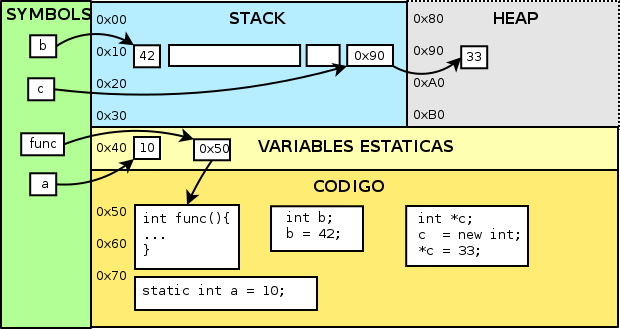
\includegraphics[width=.95\linewidth]{images/progmemoria}
\end{center}
}


\frame[containsverbatim]
{
\frametitle{Variables dinámicas de stack}

\begin{itemize}
\item Se asignan dinámicamente a memoria cuando se ejecuta el ámbito y la declaración asociada. 
\item Se liberan cuando termina su ámbito.
\item Soportan bien la recursión.
\item \textbf{Ámbitos:} procedimento, función, método, bloque.
\item En C, variables definidas en una función (variables automáticas). 
\begin{exampleblock}{C}
\begin{lstlisting}[language=C, basicstyle=\tiny, escapeinside={|}{|}]
int fun() {
    int a; // Acá se crea
    {
       float b; //Acá se crea
    }//Acá se destruye b
} // Acá se destruye a
\end{lstlisting}
\end{exampleblock}

\end{itemize} 
%ESQUEMA DE MEMORIA!!!! CODIGO -> DATOS ESTATICOS (e.g. var globales) -> stack -> heap.
}

\begin{frame}[fragile]{Dirección de Memoria}

{
\frametitle{Ejemplo}
\begin{center}
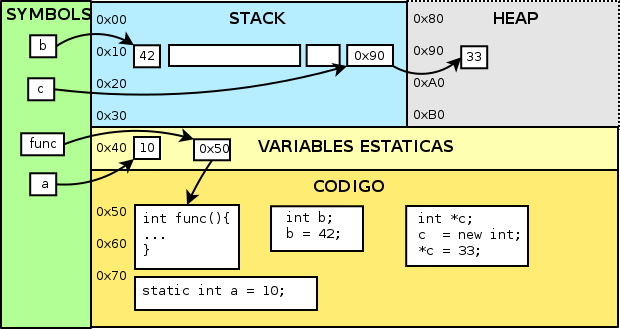
\includegraphics[width=.95\linewidth]{images/progmemoria}
\end{center}
}
\end{frame}


\section{Punteros}
\frame[containsverbatim]
{\small
\frametitle{Punteros en C}
\begin{itemize}
\item Variables de stack, que guardan \textbf{direcciones de memoria}.
\item Peso uniforme en sistemas modernos: 4 bytes in 32-bits, 8 bytes in 64-bits.  
\item Gestión de memoria dinámica (heap) y direccionamiento (stack/static)

\item Pero, \textbf{¿qué es una dirección de memoria?}
\end{itemize}

}

\subsection{Dirección de Memoria}
\begin{frame}[fragile]{Dirección de Memoria o Referencia}

\begin{itemize}
\item Las variables de stack son cajones que pueden guardar valores, pero ¿dónde están esos cajones?. 

\begin{exampleblock}{C}
\begin{lstlisting}[language=C, basicstyle=\scriptsize, escapeinside={|}{|}]
#include<stdio.h>

int main(){
	int b;
	scanf("|\%|d", &b); //¿Por qué &b?

	return 0;
}
\end{lstlisting}
\end{exampleblock}

\item El operador \& (dirección de, o referencia) nos entrega la ubicación de memoria donde se encuentra el cajón.
\end{itemize}
\end{frame}

\begin{frame}[fragile]{Analogía - Biblioteca}

\begin{center}

\includegraphics[width=.8\linewidth]{images/label}
\end{center}


\begin{itemize}
\item Va a devolver el libro \textit{\textbf{¿Cómo pasar EDA sin morir en el intento?}}.
\item Éste va en el casillero \textbf{Problema de Universitarios}.
\end{itemize}
\end{frame}

\begin{frame}[fragile]{Analogía - Biblioteca}

\begin{center}

\includegraphics[width=.8\linewidth]{images/label}
\end{center}


\begin{itemize}
\item Valor \texttt{320} como identificador del libro. \pause
\item \texttt{pu} \pause $\rightarrow$ \pause Casillero. \pause
\item \texttt{\&pu} \pause $\rightarrow$ \pause Ubicación Casillero \pause $\rightarrow$ \pause Pasillo 3, Estante 2, Fila 4. 
\end{itemize}
\end{frame}

\begin{frame}[fragile]{Analogía - Biblioteca}

\begin{center}

\includegraphics[width=.8\linewidth]{images/label}
\end{center}


\begin{itemize}
\item \texttt{pu = 320;} Bibliotecario (programador) sabé donde está el casillero. 
\item \texttt{scanf("\%d", \&pu);} Lector no sabe donde está el casillero \pause $\rightarrow$ \pause el bibliotecario le indica.
\end{itemize}
\end{frame}

\subsection{Punteros}
\frame[containsverbatim]
{\small
\frametitle{Punteros en C}
\begin{itemize}
\item Se definen con el modificador \textbf{*}, e indicando su tipo.
\begin{exampleblock}{C}
\begin{lstlisting}[language=C, basicstyle=\tiny, escapeinside={|}{|}]
int utfsm1 = 1680; //Dos variables de tipo int.
int utfsm2 = 3939; 

int *dir = NULL; //Puntero a un int, parte en NULL
//un puntero guarda la dirección de memoria de una
//variable o segmento de memoria de tipo int.
\end{lstlisting}
\end{exampleblock}

\item Diremos que un puntero \textbf{apunta} a la dirección de memoria que almacena.
\end{itemize}

}

\frame[containsverbatim]
{
\frametitle{Valor NULL}
\begin{itemize}
\item La buena práctica es inicializar los punteros hacia el vacío: el valor especial \textbf{nulo} (NULL).
\begin{exampleblock}{C}
\begin{lstlisting}[language=C, basicstyle=\tiny, escapeinside={|}{|}]
//Inicializado como puntero nulo:
double *d = NULL;
\end{lstlisting}
\end{exampleblock}
\item Aplicaciones de punteros:
\begin{itemize}
\item \textbf{Gestión dinámica de memoria:} acceso a la memoria dinámica de heap (limitada por el computador), comparado con el stack (memoria de espacio limitado). Proximamente.
\item \textbf{Direccionamiento indirecto:} útil para diseñar estructuras de datos. ELO320 en sí. 
\item \textbf{Paso por referencia:} pasar elementos por su dirección en memoria para modificarlos donde sea. Se copia dirección y no valor. Próx. Clase!
\end{itemize}
\end{itemize}
}

\subsection{Desreferencia}
\frame[containsverbatim]
{\small
\frametitle{Punteros en C}
\begin{itemize}
\item Operador de desreferencia (*): accede al valor en la dirección de memoria \textbf{a la que apunta} un puntero.
\item Los operadores * y \& son opuestos.
\item Especificador de punteros: \%p.
\item \emph{void*}: comodín para apuntar a cualquier tipo (coerción, casting).
\begin{exampleblock}{C}
\begin{lstlisting}[language=C, basicstyle=\tiny, escapeinside={|}{|}]
int utfsm1 = 1680; //Dos variables de tipo int.
int utfsm2 = 3939; 

int *dir = NULL;
dir = &utfsm1; //Puntero a un int, apunta a donde está utfsm1

printf("Dirección dentro de dir: |\%|p\n", dir);
printf("Valor dir: |\%|d\n", *dir);
printf("Dirección de dir: |\%|p\n", &dir);
\end{lstlisting}
\end{exampleblock}

\item Nota: los punteros también tienen su propia dirección de memoria (son variables!).

\end{itemize}

}

\frame[containsverbatim]
{\small
\frametitle{Punteros en C}
\begin{itemize}
\item El símbolo * no significa lo mismo dependiendo de si es definición, asignación o implementación.
\begin{exampleblock}{C}
\begin{lstlisting}[language=C, basicstyle=\tiny, escapeinside={|}{|}]

float b = 1.0; 
float * ptr; // * de declaración, solo indicamos que ptr
	     // almacena una dirección de memoria de un float

ptr = &b; // sin *, modificamos la direccion a la que apunta ptr. 

*ptr = 5.0; // * de desreferencia, se cambia el valor guardado 
	    // en la dirección de memoria apuntada por ptr

b = *ptr + 1.0; // * de desreferencia, lo que hay guardado donde se apunta + 1.0 

float * ptr2 = ptr; // * de declaración. 


\end{lstlisting}
\end{exampleblock}
\end{itemize}
}


\begin{frame}[fragile]{Analogía - Biblioteca}

\begin{center}

\includegraphics[width=.8\linewidth]{images/label}
\end{center}


\begin{itemize}
\item Preguntamos al bibliotecario o al PC de biblioteca \textbf{¿dónde está?} el libro \textbf{¿Cómo pasar EDA y MAT023 al mismo tiempo?}. 
\item Obtenemos la \textbf{dirección de la ubicación} del libro.
\item Nos dirigimos a esa dirección $\rightarrow$ \textbf{derreferencia}.
\end{itemize}
\end{frame}

\begin{frame}[fragile]{Analogía - Biblioteca}

\begin{center}

\includegraphics[width=.8\linewidth]{images/label}
\end{center}


\begin{itemize}
\item Valor 321 como identificador del libro. \pause
\item \texttt{int * ubi;} \pause $\rightarrow$ \pause puntero al libro.\pause 
\item \textbf{ubi} \pause $\rightarrow$ \pause Pasillo 3, Estante 3, Fila 1.\pause
\item \textbf{*ubi} \pause $\rightarrow$ \pause 321. 
\end{itemize}
\end{frame}


\frame[containsverbatim]
{
\frametitle{Aritmética de Punteros}
\begin{itemize}
\item Indicar el tipo a un puntero sirve para realizar aritmética de punteros.
\item Transforma 1 unidad decimal, en 1 unidad segun el tamaño del tipo. 
\item Podemos saber cuanta memoria hay entre un puntero y el siguiente (si es que existe).
\item Ejemplo: Puntero a int avanza de a 4 bytes.
\end{itemize}
\begin{exampleblock}{C}
\begin{lstlisting}[language=C, basicstyle=\tiny, escapeinside={|}{|}]
float num = 2.5;
float *f;
f = &num; //Dirección a num.

printf("Direccion f: |\%|p\n", f); //¿Cuál es la diferencia
printf("Direccion f+1: |\%|p\n", f+1); //entre f y f+1?
\end{lstlisting}
\end{exampleblock}
\begin{itemize}
\item Respuesta: La diferencia es de 4 bytes (tamaño de float).
\end{itemize}

}

\frame[containsverbatim]
{
\frametitle{Arreglos y Aritmética de Punteros}
\begin{itemize}
\item En C un arreglo puede trabajarse con aritmética de punteros.
\item Esto se debe a que los arreglos son compatibles con los punteros.
\item El compilador hace coerción y esto permite el uso de la aritmética de punteros.
\begin{exampleblock}{C}
\begin{lstlisting}[language=C, basicstyle=\tiny, escapeinside={|}{|}]
int a[10], i;
int *pa, *pb;
pa = &a[0]; /* dir. elemento 0 de arreglo a. tamaño 1 int */
pa = a;	    /* hace lo mismo que la linea anterior con coerción */
pb = &a;    /* dir. de arreglo a. tamaño 10 int */

for (i=0; i<10; i++){
	printf("|\%|d ", a[i]);
	printf("|\%|d ", *(pa+i));
	printf("|\%|d ", *(a+i));
}
/* los tres for hacen lo mismo */

printf(printf("|\%|d ", *(pb+1)); //¿Qué pasa acá?
\end{lstlisting}
\end{exampleblock}
\end{itemize}
}




\section{Paso por Valor y Paso por Referencia}
\frame[containsverbatim]
{
  \frametitle{Funciones y Punteros: Paso por Valor}
  \small
  \begin{itemize}
  \item Los parametros copian los valores que fueron pasados como parámetros. 
  \item Las variables originales se mantienen inalteradas.
  \end{itemize}
\begin{exampleblock}{C}
\begin{lstlisting}[language=C, basicstyle=\tiny, escapeinside={|}{|}]
#include<stdio.h>

void swap(int a, int b){
	int temp;
	temp = a;
	a = b;
	b = temp;
}

int main(){
	int x=2, y=3;
	swap(x,y);
	printf("x: |\%|d, y: |\%|d\n", x, y); //¿Qué imprime?
	return 0;
}

\end{lstlisting}
\end{exampleblock}
}

\frame[containsverbatim]
{
  \frametitle{Funciones y Punteros: Paso por Referencia}
  \small
  \begin{itemize}
  \item Los parametros son punteros locales, pero la derreferencia es la misma local o global.
  \item Las variables originales se modifican.
  \end{itemize}
\begin{exampleblock}{C}
\begin{lstlisting}[language=C, basicstyle=\tiny, escapeinside={|}{|}]
#include<stdio.h>

void swap(int *a, int *b){ //punteros locales
	int temp;
	temp = *a; //se guarda lo que hay donde apunta a
	*a = *b; //cambio entre los valores donde apuntan los punteros
	*b = temp; //agrego valor guardado, no se cambian los punteros, ojo.
}

int main(){
	int x=2, y=3;
	swap(|\&|x,|\&|y);
	printf("x: |\%|d, y: |\%|d\n", x, y); //¿Qué imprime?
	return 0;
}

\end{lstlisting}
\end{exampleblock}
}


\frame[containsverbatim]
{
  \frametitle{Funciones y Punteros: Paso por Referencia}
  \small
  \begin{itemize}
  \item ¿Funciona este tercer caso?
  \end{itemize}
\begin{exampleblock}{C}
\begin{lstlisting}[language=C, basicstyle=\tiny, escapeinside={|}{|}]
#include<stdio.h>

void swap(int *a, int *b){ //punteros locales
	int *temp;
	temp = a; 
	a = b; 
	b = temp;
}

int main(){
	int x=2, y=3;
	swap(|\&|x,|\&|y);
	printf("x: |\%|d, y: |\%|d\n", x, y); //¿Qué imprime?
	return 0;
}

\end{lstlisting}
\end{exampleblock}
\begin{itemize}
\item Respuesta: No, no funciona. Punteros locales. 
\end{itemize}
}


\frame[containsverbatim]
{
  \frametitle{Funciones y Punteros: Paso por Referencia}
  \small
  \begin{itemize}
  \item ¿Funciona este cuarto caso?
  \end{itemize}
\begin{exampleblock}{C}
\begin{lstlisting}[language=C, basicstyle=\tiny, escapeinside={|}{|}]
#include<stdio.h>

void swap(int *a, int *b){ //punteros locales
	int *temp;
	temp = a; 
	*a = *b; 
	*b = *temp;
}

int main(){
	int x=2, y=3;
	swap(|\&|x,|\&|y);
	printf("x: |\%|d, y: |\%|d\n", x, y); //¿Qué imprime?
	return 0;
}
\end{lstlisting}
\end{exampleblock}
\begin{itemize}
\item Respuesta: No, se pierde el valor de *a.
\end{itemize}
}


\end{document}
